
%% bare_conf.tex
%% V1.3
%% 2007/01/11
%% by Michael Shell
%% See:
%% http://www.michaelshell.org/
%% for current contact information.
%%
%% This is a skeleton file demonstrating the use of IEEEtran.cls
%% (requires IEEEtran.cls version 1.7 or later) with an IEEE conference paper.
%%
%% Support sites:
%% http://www.michaelshell.org/tex/ieeetran/
%% http://www.ctan.org/tex-archive/macros/latex/contrib/IEEEtran/
%% and
%% http://www.ieee.org/

%%*************************************************************************
%% Legal Notice:
%% This code is offered as-is without any warranty either expressed or
%% implied; without even the implied warranty of MERCHANTABILITY or
%% FITNESS FOR A PARTICULAR PURPOSE! 
%% User assumes all risk.
%% In no event shall IEEE or any contributor to this code be liable for
%% any damages or losses, including, but not limited to, incidental,
%% consequential, or any other damages, resulting from the use or misuse
%% of any information contained here.
%%
%% All comments are the opinions of their respective authors and are not
%% necessarily endorsed by the IEEE.
%%
%% This work is distributed under the LaTeX Project Public License (LPPL)
%% ( http://www.latex-project.org/ ) version 1.3, and may be freely used,
%% distributed and modified. A copy of the LPPL, version 1.3, is included
%% in the base LaTeX documentation of all distributions of LaTeX released
%% 2003/12/01 or later.
%% Retain all contribution notices and credits.
%% ** Modified files should be clearly indicated as such, including  **
%% ** renaming them and changing author support contact information. **
%%
%% File list of work: IEEEtran.cls, IEEEtran_HOWTO.pdf, bare_adv.tex,
%%                    bare_conf.tex, bare_jrnl.tex, bare_jrnl_compsoc.tex
%%*************************************************************************
%

\documentclass[conference]{IEEEtran}

\usepackage{graphicx}
\usepackage{color}
\usepackage{multirow}


%\graphicspath{{fig/}}
\newcommand \todo[1]{\textcolor{red}{\textsl{TODO: }}{\textcolor{black}{#1}}}
\newcommand \modified[1]{{\textcolor{black}{#1}}}

\hyphenation{op-tical net-works semi-conduc-tor}

\graphicspath{ {../../figures/} }

\begin{document}

\title{White Rabbit: a PTP Application for Robust Sub-nanosecond Synchronization}

% author names and affiliations
% use a multiple column layout for up to three different
% affiliations

\author{

%\IEEEauthorblockN{Bunch of Freaks}
%\IEEEauthorblockA{CERN\\
%Geneva\\
%Email: white.rabbit@cern.ch}

\IEEEauthorblockN{Maciej Lipi\'{n}ski, Tomasz W\l{}ostowski, Javier Serrano, Pablo Alvarez}
\IEEEauthorblockA{CERN, Geneva\\
Email: \{maciej.lipinski, tomasz.wlostowski, javier.serrano, pablo.alvarez.sanchez\}@cern.ch}

}

% conference papers do not typically use \thanks and this command
% is locked out in conference mode. If really needed, such as for
% the acknowledgment of grants, issue a \IEEEoverridecommandlockouts
% after \documentclass

% for over three affiliations, or if they all won't fit within the width
% of the page, use this alternative format:
% 
%\author{\IEEEauthorblockN{Michael Shell\IEEEauthorrefmark{1},
%Homer Simpson\IEEEauthorrefmark{2},
%James Kirk\IEEEauthorrefmark{3}, 
%Montgomery Scott\IEEEauthorrefmark{3} and
%Eldon Tyrell\IEEEauthorrefmark{4}}
%\IEEEauthorblockA{\IEEEauthorrefmark{1}School of Electrical and Computer
%Engineering\\
%Georgia Institute of Technology,
%Atlanta, Georgia 30332--0250\\ Email: see
%http://www.michaelshell.org/contact.html}
%\IEEEauthorblockA{\IEEEauthorrefmark{2}Twentieth Century Fox, Springfield,
%USA\\
%Email: homer@thesimpsons.com}
%\IEEEauthorblockA{\IEEEauthorrefmark{3}Starfleet Academy, San Francisco,
%California 96678-2391\\
%Telephone: (800) 555--1212, Fax: (888) 555--1212}
%\IEEEauthorblockA{\IEEEauthorrefmark{4}Tyrell Inc., 123 Replicant Street, Los
%Angeles, California 90210--4321}}


\maketitle

\begin{abstract}

White Rabbit (WR) is a time-deterministic, low-latency Ethernet-based network which enables 
transparent, sub-ns accuracy timing distribution. It is being developed to replace 
the General Machine Timing (GMT) 
%\cite{biblio:GMT} 
system currently used at CERN and will become 
the foundation for the control system of the Facility for Antiproton and Ion Research (FAIR) 
at GSI. High reliability is an important issue in WR's design, 
since unavailability of the accelerator's 
control system will directly translate into expensive downtime of the machine. 
A typical WR network is required to lose not more than a single message per year. 
Due to WR's complexity, the translation of this real-world-requirement into 
a reliability-requirement constitutes an interesting issue on its own -- a WR network 
is considered functional only if it provides all its services to all its clients at any time. 
This paper defines reliability in WR and describes how it was addressed by dividing it into 
sub-domains: deterministic packet delivery, data 
%redundancy, 
resilience, 
topology redundancy and clock 
resilience. The studies show that the Mean Time Between Failure (MTBF) of the WR Network 
is the main factor affecting its reliability. Therefore, probability calculations for 
different topologies were performed using the "Fault Tree analysis" and analytic estimations. 
Results of the study show that the requirements of WR are demanding. Design changes might be needed 
and further in-depth studies required, e.g. Monte Carlo simulations. Therefore, a direction 
for further investigations is proposed.
\end{abstract}


% \begin{IEEEkeywords}
% IEEE 1588 Precision Time Protocol (PTP); Synchronous Ethernet; frequency syntonization; time
% synchronization; network redundancy;


% IEEE 1588 Precision Time Protocol (PTP)
% Synchronous Ethernet
% --------------------
% Ethernet networks
% Next generation networking
% Optical fiber networks
% Real time systems
% Time measurement
% Phase frequency detector
% Networked control systems
% Redundancy
% Determinism
% -----------------------

% \end{IEEEkeywords}
%% For peer review papers, you can put extra information on the cover
% page as needed:
% \ifCLASSOPTIONpeerreview
% \begin{center} \bfseries EDICS Category: 3-BBND \end{center}
% \fi
%
% For peerreview papers, this IEEEtran command inserts a page break and
% creates the second title. It will be ignored for other modes.
\IEEEpeerreviewmaketitle

\section{Introduction}

White Rabbit (WR, \cite{biblio:whiteRabbit}) is a project which aims at creating an
Ethernet-based network with low-latency, deterministic packet delivery
and network-wide, transparent, high-accuracy timing distribution. The
White Rabbit Network (WRN) is based on existing standards, namely
Ethernet (IEEE 802.3 \cite{biblio:IEEE8023}), Synchronous Ethernet
(SyncE \cite{biblio:SynchE}) and PTP \cite{biblio:IEEE1588}. 
It is fully compatible with these standards.

A WRN consists of White Rabbit Nodes (nodes) and White Rabbit Switches
(switches) interconnected by fiber or copper links. 
\modified{The focus of this article is on 1000Base-LX \cite{biblio:IEEE1588} 
single-mode fiber connections only. WR }%It also
supports integration of nodes and/or switches that are not White Rabbit. 
A simple WRN is presented in \figurename~\ref{fig:WRnetwork}.

A node is considered the source and destination of information sent
over the WRN. The information distributed over a WRN includes:
\begin{itemize}
   \item  Timing - frequency and International Atomic Time (TAI).
   \item  Data  - Ethernet traffic between nodes.
\end{itemize} 

In order to understand the goals of the WR project -- namely
determinism, high reliability and accurate synchronization -- these
terms are explained below.

\textbf{Determinism} is guaranteed by having a worst-case upper bound
in frame delivery latency.  

\textbf{Accuracy} is a measure of the deviation between the clock of
the \textit{grandmaster} node\modified{/switch} of a WRN and that of any other node.
Assuming only fiber interconnections, a WRN is meant to achieve
sub-nanosecond accuracy. 

\textbf{Reliability} of a WRN refers to robust delivery of data and
timing to all the nodes.
% data being delivered in a deterministic manner. 
%A WRN is considered reliable only if all the nodes, receive
%data and timing. 
The timing must allow all the nodes to be
synchronized with the required accuracy and the data must always be
delivered on time.
\begin{figure}[!t]
\centering
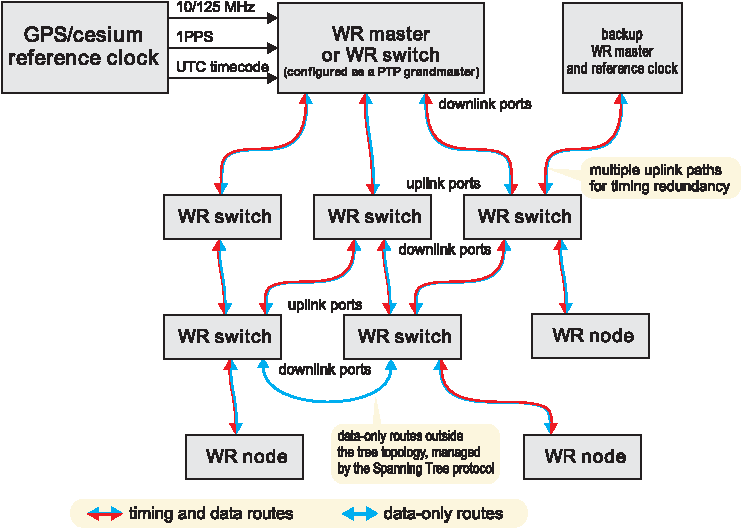
\includegraphics[height=2.10in]{../../figures/network/hierarchy.eps}
\caption{A White Rabbit Network \cite{biblio:TomekMSc}.}
\label{fig:WRnetwork}
\end{figure}

All these features are required to create a timing and control system which may
replace the General Machine Timing (GMT) \cite{biblio:GMT} at CERN and
fulfill a similar role at the Facility for Antiproton and Ion
Research (FAIR) in GSI \cite{biblio:FAIRtimingSystem}. Such system requires 
synchronization of up to 2000 nodes with sub-nanosecond accuracy, 
an upper bound in frame delivery and a very low data loss rate.
However, many other applications of White Rabbit are possible. This includes industry,
telecommunications and other large distributed systems (e.g. distributed
oscilloscopes \cite{biblio:distOscilloscope}).

This article focuses solely on the PTP-based timing distribution in a WRN. PTP is a packet-based
protocol designed to synchronize devices in distributed systems. The accuracy of the PTP
synchronization is implementation-dependent. The standard is foreseen for 
% this is how I understand the fact that corretionField can carry fractional
% nanoseconds and the syncEventEgressTimestamp includes this figures (see e.g.: 
% clause 9.5.9.3, page 103 of PTP
sub-nanosecond accuracies. However, such performance is not achieved in typical PTP
implementations for two reasons:
\begin{itemize}
  \item Limited precision and resolution of PTP timestamps.
  \item Unknown physical link asymmetry. 
\end{itemize}
Additionally, the quality of PTP-syntonization depends on the exchange rate 
of PTP messages. The higher the quality of the clock we want to recover, 
the higher the bandwidth needed for PTP-related traffic.

The precision of timestamps is greatly increased in the existing PTP implementations
by hardware-based timestamping. However, such implementations
are limited by the resolution which is specified by the hardware-driving frequency
(e.g. 8ns for 125MHz).

The asymmetry is not detectable by PTP; if known, PTP corrects for it to increase
synchronization accuracy. Some of the sources of the physical layer asymmetry can be
eliminated by proper network configuration, e.g. excluding routers or non-PTP bridges from the
network. Others, in particular the inaccuracy caused by physical medium asymmetry (i.e.
difference in propagation velocity in two-way communication over fiber) or PCB layout (i.e.
connection length between PHY and timestamping hardware) need to be obtained through proper a
priori-measurement. 

White Rabbit addresses these limitations to achieve sub-nanosecond accuracy
of synchronization. It uses SyncE to distribute the common notion of frequency in the entire
network over the physical medium. It casts the problem of timestamping into a phase detection
measurement. The results of these precise measurements are used both during normal PTP operation
and for quantifying physical medium asymmetry during the calibration phase.
% Consequently, high precision
% timestamps are obtained. Moreover, the parameters necessary to calculate the physical medium
% asymmetry can be determined. 
%This knowledge is used in the PTP computations of the clock offset and link delay. 
The improved performance of the synchronization is accomplished without increasing PTP-related
traffic (it can be actually decreased) since PTP is only governing the synchronization, while the
syntonization is done by SyncE.

A great effort has been made to align WR-specific solutions with the PTP standard and stay fully
compatible with PTP gear. Consequently, WR can be seen as an extension to PTP. This extension,
called WRPTP, defines its own PTP profile and describes all the WR-specific mechanisms which need
to be implemented by a node/switch to enable sub-nanosecond synchronization with another 
nodes/switches. 
\modified{The compatibility with PTP makes WR more likely to be used in existing PTP-based 
systems by gradual and/or partial upgrade to WRPTP. It also enables the creation of hybrid, 
thus cost-effective, systems.}
WRPTP is presented in section~\ref{sec:wrptp} \textit{White Rabbit PTP}.
Section~\ref{sec:hwSupport} presents an example implementation of 
hardware which supports WRPTP. Finally, the measurements of WRPTP performance and conclusions are
presented in the last two sections of this article.

In PTP nomenclature, the main component of a WRN, the switch, is a boundary clock (BC) -- a clock 
that has multiple PTP ports. Similarly, the node is an ordinary clock (OC) --
a clock that has a single PTP port. Consequently, the WRN
can be seen as a set of independently synchronized Master-to-Slave
(M-to-S) links with ports of OC or BC on both sides
(\figurename~\ref{fig:WRnetwork}, red-blue arrows). The ability to
synchronize a single link scales into the ability to synchronize the
entire network. Therefore, in this article, only a single M-to-S link is
considered, where appropriate.




\section{White Rabbit extension to PTP (WRPTP)}
\label{sec:wrptp}

White Rabbit extends the PTP standard benefiting from PTP's mechanisms, 
taking advantage of its customization facilities (i.e. PTP profiles
and Type-Length-Value, TLV) but also defining implementation-specific 
functionalities and staying PTP-compatible. 

% \begin{figure}[!t]
% \centering
% 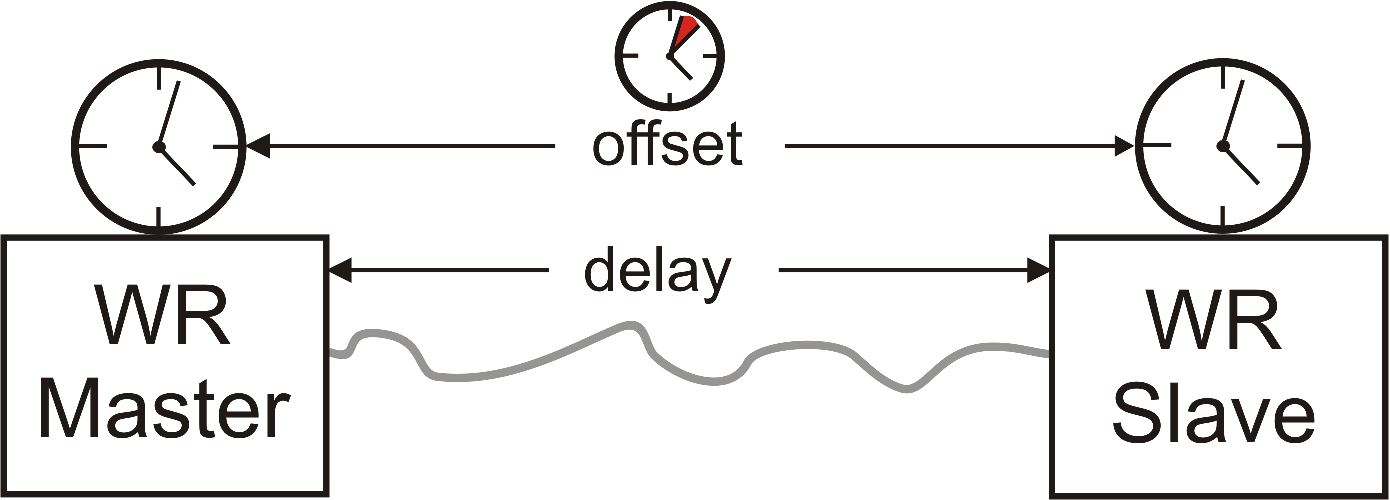
\includegraphics[width=3in]{fig/wrLink.eps}
% \caption{WR Link \modified{Delay} Model, synchronization and syntonization scheme.}
% \label{fig:wrLink}
% \end{figure}

\begin{figure}[!t]
\centering
\includegraphics[width=3.15in]{protocol/wrptpMSGs.eps}
\caption{\modified{Simplified overview of the message flow in WRPTP.}}
\label{fig:wrptpMSGs}
\end{figure}

WRPTP introduces the \textit{WR Link Setup} (section~\ref{sec:wrLinkSetup}) process which
provides inputs to the \textit{WR Link \modified{Delay} Model} (section~\ref{sec:wrLinkModel}) 
to obtain accurate delay and offset calculations. 
The WR Link Setup is a process for establishing the WR link. It includes WR node
identification, syntonization, measurement of WR-specific parameters and 
their distribution over the link. The additional communication during the WR Link Setup 
is done through extended PTP messaging facilities (section~\ref{sec:wrMessages}). 
The WR-specific parameters, which are exchanged and set during this process, are 
stored in WR-specific data set fields (section~\ref{sec:wrDataSet}). 

The flow of events for the standard PTP is extended as depicted in \figurename~\ref{fig:wrptpMSGs}
and described below:

\begin{enumerate}
\item \textbf{WR Port A} which is in PTP\_MASTER state periodically sends WR Announce messages
      (section~\ref{sec:wrMessages}).
\item \textbf{WR Port B} receives Announce message(s), recognizes the WR Announce message and 
      uses the modified Best Master Clock (mBMC) algorithm (section~\ref{sec:wrBMC}) to establish its
      place in the WR network hierarchy.
\item \textbf{WR Port B} enters WR Slave mode (based on the conditions in 
      \ref{sec:wrLinkSetup}) and starts the WR Link Setup by sending the M\_SLAVE\_PRESENT message.
\item \textbf{WR Port A} enters WR Master mode (based on the conditions in 
      \ref{sec:wrLinkSetup}) and sends the M\_LOCK message to request the WR Slave to start
      syntonization.
\item The WR Slave sends the M\_LOCKED message as soon as the syntonization process is 
      finished.
\item The WR Master sends the M\_CALIBRATE message to request a calibration pattern in order to 
      measure its reception fixed delay.
\item The WR Master sends the M\_CALIBRATED message as soon as the calibration is 
      finished.
\item The WR Slave sends the M\_CALIBRATE message to request a calibration pattern in order to 
      measure its reception fixed delay.
\item The WR Slave sends the M\_CALIBRATED message as soon as the calibration is 
      finished.
\item The WR Master sends the M\_WR\_MODE\_ON message to indicate completion of  the WR
      Link Setup process.
\item PTP two-step clock request-response delay measurement is performed repeatedly ($t_{1}$,
      $t_{2}$, $t_{3}$, $t_{4}$). WR Slave calculates M-to-S delay and clock offset and adjusts its
      time counters.
\end{enumerate}

% \begin{figure}[!t]
% \centering
% \includegraphics[width=3.5in]{fig/wrptpMSGs.eps}
% \caption{\modified{Simplified overview of the message flow in WRPTP.}}
% \label{fig:wrptpMSGs}
% \end{figure}

\begin{figure}[!t]
\centering
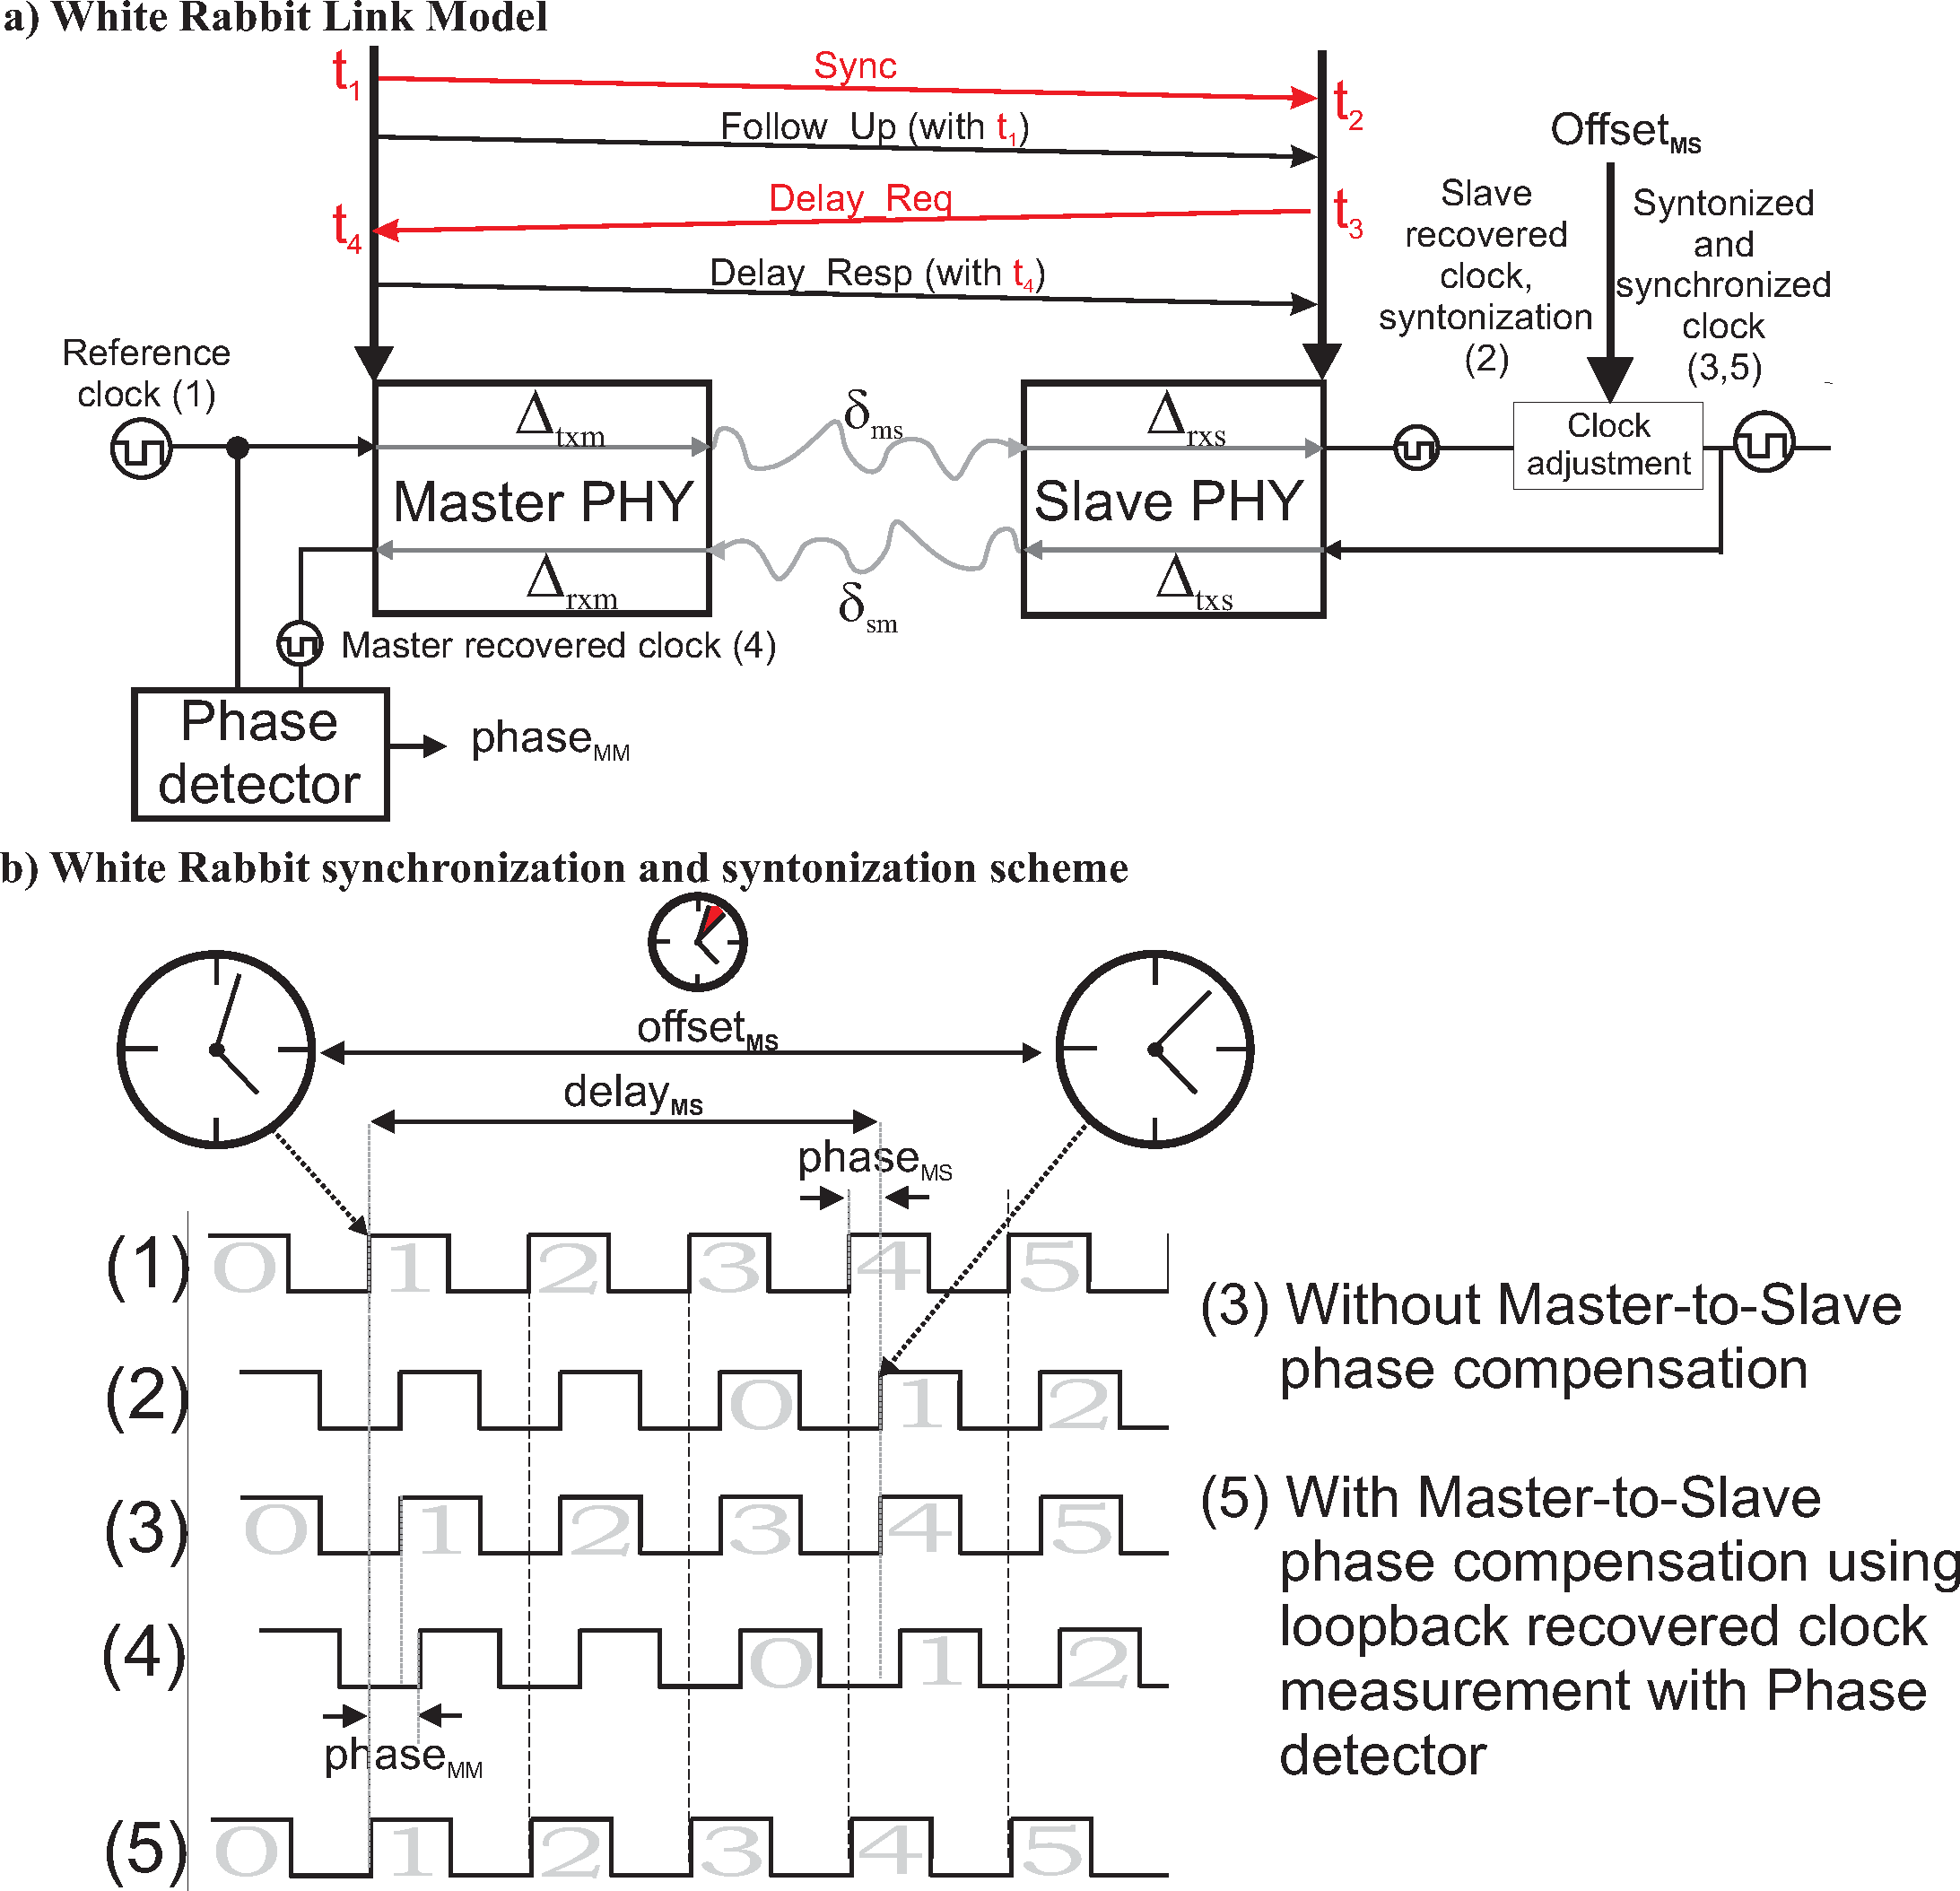
\includegraphics[width=3.1in]{protocol/wrLink2.eps}
\caption{WR Link \modified{Delay} Model, synchronization and syntonization scheme.}
\label{fig:wrLink}
\end{figure}



%%%%%%%%%%%%%%%%%%%%%%%%%%%%%%%%%%%%%%%%%%%%%%%%%%%%%%%%%%%%%%%%%%%%%%%%%%%%%%%
%             WR Link Delay Model
%%%%%%%%%%%%%%%%%%%%%%%%%%%%%%%%%%%%%%%%%%%%%%%%%%%%%%%%%%%%%%%%%%%%%%%%%%%%%%%

\subsection{WR Link \modified{Delay} Model}
\label{sec:wrLinkModel}
Sub-nanosecond synchronization requires a precise knowledge of one-way 
M-to-S delay ($ delay_{ms}$). PTP measures 
the round-trip delay ($delay_{MM}$). Usually, delay symmetry 
($delay_{ms}=delay_{sm}$) is assumed to derive the one-way delay. In
White Rabbit, the \textit{WR Link \modified{Delay} Model} (\figurename~\ref{fig:wrLink}, (a)) 
is used to calculate the precise M-to-S delay by including link asymmetry. 
The delay can be expressed as the sum:
\begin{equation}
  \label{eq:delayms}
  delay_{ms} = \Delta_{tx_m} + \delta_{ms} + \Delta_{rx_s}
\end{equation}
where $\Delta_{tx_m}$ is the fixed delay due to the master's
transmission circuitry, $\delta_{ms}$ is the variable delay of the
transmission medium and $\Delta_{rx_s}$ is the fixed circuitry
reception delay in the slave. Similarly, the S-to-M
delay ($ delay_{sm}$) can be described using $\Delta_{tx_s}$,
$\delta_{sm}$ and $\Delta_{rx_m}$ respectively. The fixed delays
($\Delta_{rx_s,tx_s,rx_m,tx_m}$) are considered constant for a given
connection. They can be measured by nodes/switches at the beginning of 
the connection, as described in section~\ref{sec:TxRxLatencies}. For
highest precision, WR uses a single fiber for two-way
communication -- the asymmetry is directly and solely caused
by the difference in propagation velocity in both directions. Consequently, the
difference between $\delta_{ms}$ and $\delta_{sm}$ is connected to the
wavelength difference for transmitting and receiving the data
(e.g. 1550 and 1310 nm). The equation describing the relation between
$\delta_{ms}$ and $\delta_{sm}$ is defined in \cite{biblio:WRPTP}.
For bi-directional fiber, it is governed by the 
\textit{relative delay coefficient~($\alpha$)}:
\begin{equation}
  \label{eq:alpha}
  \alpha = \frac{\delta_{ms}}{\delta_{sm}}-1 = \frac{n_{1550}}{n_{1310}}-1
\end{equation}
The $\alpha$ coefficient can be calculated using refractive indexes
($n_{1550}$, $n_{1310}$) or, preferably, measured for a given fiber type. 

Knowing the coefficient, the round-trip delay ($delay_{MM}$)
and the fixed delays ($\Delta_{rx_s,tx_s,rx_m,tx_m}$), 
the precise M-to-S delay (\ref{eq:delayMS}) can be calculated using (\ref{eq:delta}) and
(\ref{eq:ptpTimestamps}). See \cite{biblio:WRPTP} and
\cite{biblio:TomekMSc} for a detailed derivation.
\begin{equation}
\label{eq:delta}
  \Delta = \Delta_{tx_m} + \Delta_{rx_s} + \Delta_{tx_s} + \Delta_{rx_m}
\end{equation}
\begin{equation}
\label{eq:ptpTimestamps}
  delay_{MM} =  \Delta + \delta_{ms} +\delta_{sm}
\end{equation}
\begin{equation}
\label{eq:delayMS}
  delay_{ms} = \frac{1 + \alpha}{2 + \alpha}(delay_{MM}-\Delta)
\end{equation}
Finally, the value of the offset ($offset_{ms}$) between the master's
clock and that of the slave is obtained (\ref{eq:offset}). It is fed
into the adjustment algorithm of the slave's clock servo
(\figurename~\ref{fig:wrLink}).
\begin{equation}
\label{eq:offset}
  offset_{ms} = t_1-t_{2p} - delay_{ms}
\end{equation}
The $t_{2p}$ in (\ref{eq:offset}) is the enhanced-precision value of PTP $t_2$ 
which is obtained during the \textit{Fine Delay Measurement} described
in section~\ref{sec:fineDelay}. The same process is used to obtain a very precise
value of $t_{4}$.
% The fixed delays ($\Delta_{rx_s,tx_s,rx_m,tx_m}$) measurement is described in 
% section~\ref{sec:TxRxLatencies}.

% \modified{The link asymmetry, thus the precise one-way delay, 
% is re-evaluated periodically each time new PTP-timestamps are obtained. It enables to compensate for 
% the possible changes of the link characteristics.}
%The application of the \textit{WR Link \modified{Delay} Model} needs extensions to the
%PTP standard which are described in the next sub-section.


%%%%%%%%%%%%%%%%%%%%%%%%%%%%%%%%%%%%%%%%%%%%%%%%%%%%%%%%%%%%%%%%%%%%%%%%%%%%%%%
%             WR Data Sets
%%%%%%%%%%%%%%%%%%%%%%%%%%%%%%%%%%%%%%%%%%%%%%%%%%%%%%%%%%%%%%%%%%%%%%%%%%%%%%%

\subsection{WR Data Sets}
\label{sec:wrDataSet}

WRPTP adds fields to the data sets defined in the PTP standard 
%(\tablename~\ref{tab:wrDS}) % table excluded from article due to the lack of space and uselessnes
and defines a new data set (backupParentDS) to store WR-specific parameters. All new fields, except
\textit{primarySlavePortNumber}, are added to the \textit{portDS} data set. 
The \textit{primarySlavePortNumber} field is added to the \textit{currentDS} data set.

% \begin{table}[!t]
% %\renewcommand{\arraystrech}{1.3}
% \caption{WRPTP data sets fields (\textbf{D}=Dynamic, \textbf{S}=Static).}
% \label{tab:wrDS}
% \centering
% \begin{tabular}{| l     |     c         |  l |   }        \hline   
%    
% \textbf{DS member}     	&  \textbf{D}/\textbf{S} & \textbf{Description}\\   \hline
% %			&   &                \\ \hline
% %%%%%%%%%%%%%%%%%%%%%%%%%%%%%%%%%%%%%%%%%%%%%%%%%%%%%%%%%%%%%%%%%%%%%%%%%%%%%%%%%%%%%%%%%%
% wrConfig   		& S & predefined function of a WR port \\ \hline
% wrMode			& D & current WR mode of a WR port	 \\ \hline
% wrModeOn 		& D & mode defined in wrMode is active \\ \hline
% wrPortState 		& D & current state of the WR FSM      \\ \hline
% calibrated 		& D & fixed delays of the given port   \\ \hline
% deltaTx       		& D & port's $\Delta_{tx}$             \\ \hline
% deltaRx     		& D & port's $\Delta_{rx}$             \\ \hline
% calPeriod   		& S & calibration period\\ \hline
% %%%%%%%%%%%%%%%%%%%%%%%%%%%%%%%%%%%%%%%%%%%%%%%%%%%%%%%%%%%%%%%%%%%%%%%%%%%%%%%%%%%%%%%%%%
% parentWrConfig 		& D & wrConfig of the parent port\\ \hline
% parentWrMode		& D & wrMode of the parent port\\ \hline
% parentWrModeOn 		& D & wrModeOn of the parent port\\ \hline
% parentDeltaTx      	& D & calibrated of the parent port\\ \hline
% parentDeltaRx     	& D & deltaTx of the parent port\\ \hline
% parentCalPeriod   	& S & deltaRx of the parent port\\ \hline
% %%%%%%%%%%%%%%%%%%%%%%%%%%%%%%%%%%%%%%%%%%%%%%%%%%%%%%%%%%%%%%%%%%%%%%%%%%%%%%%%%%%%%%%%%%
% primarySlavePortNumber	&  D &port number of the Primary Slave  \\ \hline
% 
% \end{tabular}
% 
% \end{table}

%%%%%%%%%%%%%%%%%%%%%%%%%%%%%%%%%%%%%%%%%%%%%%%%%%%%%%%%%%%%%%%%%%%%%%%%%%%%%%%
%             WR Messages
%%%%%%%%%%%%%%%%%%%%%%%%%%%%%%%%%%%%%%%%%%%%%%%%%%%%%%%%%%%%%%%%%%%%%%%%%%%%%%%

\subsection{WR Messages}
\label{sec:wrMessages}

WRPTP defines a WR Type-Length-Value (WR TLV) extension to exchange the WR-specific data.
In particular, it is used to suffix Announce and create Signaling Messages. 
WR TLVs are recognized (see \tablename~35 of PTP) by the TLV type
(\textit{tlvType}=\textit{ORGANIZATION\_EXTENSION}), CERN's Organizationally Unique Identifier 
(\textit{OrganizationId} = 0x080030), magic and version numbers. The different types of WR
TLVs are distinguished by a WR Message Identifier (wrMessageID), as defined in
\tablename~\ref{tab:wrMessageId}.

\begin{table}[!t]
\caption{White Rabbit Message ID values}
\centering
\begin{tabular}{| l | c| c | c |}          \hline
\textbf{Message name}  &  \textbf{wrMessageId} &  \textbf{Sent in message type} \\   \hline
%& &  \\ \hline
M\_SLAVE\_PRESENT     &  0x1000 & Signaling \\ \hline
M\_LOCK               &  0x1001 & Signaling \\ \hline
M\_LOCKED             &  0x1002 & Signaling \\ \hline
M\_CALIBRATE          &  0x1003 & Signaling \\ \hline
M\_CALIBRATED         &  0x1004 & Signaling \\ \hline
M\_WR\_MODE\_ON       &  0x1005 & Signaling \\ \hline
M\_ANN\_SUFIX	      &  0x2000 & Announce  \\ \hline
\end{tabular}
\label{tab:wrMessageId}
\end{table}

%%%%%%%%%%%%%%%%%%%%%%%%%%%%%%%%%%%%%%%%%%%%%%%%%%%%%%%%%%%%%%%%%%%%%%%%%%%%%%%
%             WR Messages
%%%%%%%%%%%%%%%%%%%%%%%%%%%%%%%%%%%%%%%%%%%%%%%%%%%%%%%%%%%%%%%%%%%%%%%%%%%%%%%

\subsection{Modified BMC}
\label{sec:wrBMC}
The standard method of handling topology and grandmaster redundancy in a BC-based PTP network 
is not sufficient for the WRN. The BMC allows only a single port (slave) of a BC to 
be synchronized to a single grandmaster. A time source failure requires re-synchronization and might
introduce fluctuations in the notion of time.

% The BMC allows no more than one port of a BC to be in the PTP\_SLAVE state. Such a
% solution allows for redundancy of the time source and topology but is not optimal for the
% continuity of the synchronization. In case of a failure of one of the \textit{best}
% clocks, the restart of the estimation of the clock drift, mean path delay and offset is required
% which might cause fluctuations in the notion of time. 
 
The modified BMC (mBMC) allows for more than one \textit{best} clock in a single domain, 
enabling the creation of a logic topology with multiple roots. A BC 
running the mBMC can have more than one port in the PTP\_SLAVE state (slave ports). 
This means that timing information is exchanged between a BC and 
more than one source of time (i.e. OC or BC). At any time 
any of these sources can be used to perform synchronization, including a weighted 
average from all slave ports as mentioned in \cite{biblio:Takahide}.

The modification applies to the State Decision Algorithm (SDA): the BMC\_SLAVE 
recommended state is enforced instead of the BMC\_PASSIVE state 
\modified{for the clocks with clockClass greater than 127 \cite{biblio:IEEE1588}}. A port
which becomes a slave as a result of the modification, is considered
a Secondary Slave. A slave port resulting from the unchanged part of the SDA,
is considered a Primary Slave and its number is stored in the \textit{primarySlavePortNumber}. 

The best qualified Announce messages ($E_{rbest}$) 
from all Secondary Slave ports are compared using the Data Comparison Algorithm (DCA) 
to determine the "second best master" and the lower order masters. The results 
are stored in the \textit{backupParentDS} \modified{(section~\ref{sec:wrDataSet})}.

The provided information about Primary and Secondary Slaves is used by the WR hardware
to support a seamless switch-over in case of failure of the best master 
(section~\ref{sec:wrCRS}). \modified{Such a solution enables robust synchronization with no 
deterioration of its quality while switching between the redundant components.}
%%%%%%%%%%%%%%%%%%%%%%%%%%%%%%%%%%%%%%%%%%%%%%%%%%%%%%%%%%%%%%%%%%%%%%%%%%%%%%%
%             Link Setup
%%%%%%%%%%%%%%%%%%%%%%%%%%%%%%%%%%%%%%%%%%%%%%%%%%%%%%%%%%%%%%%%%%%%%%%%%%%%%%%

\subsection{WR Link Setup}
\label{sec:wrLinkSetup}

The process of establishing a White Rabbit link between two WR ports
is called \textit{WR Link Setup}. It involves the
recognition of two compatible WR ports, their WR modes assignment
(WR Master or WR Slave), syntonization over the physical layer, 
measurement of the fixed delays ($\Delta_{rx_s,tx_s,rx_m,tx_m}$) and 
exchange of their values across the link. The WR Link Setup is controlled by the
White Rabbit state machine (WR FSM) which is executed in the PTP\_UNCALIBRATED 
state of the PTP FSM \modified{on the WR Slave, and in the PTP\_MASTER state on the WR Master}. 
The WR FSM is depicted in \figurename~\ref{fig:wrFSM} and 
its usual execution on the WR Master and the WR Slave during the WR Link Setup is
presented in \figurename~\ref{fig:wrptpMSGs}.
%%%%%%%%%%%%%%%%%%%%%%%%%%%%%%%%%%%%%%%%%%%%%%%%%%%%%%%%%%%%%%%%%%%%%%%%%%%%%%%
\begin{figure}[!t]
\centering
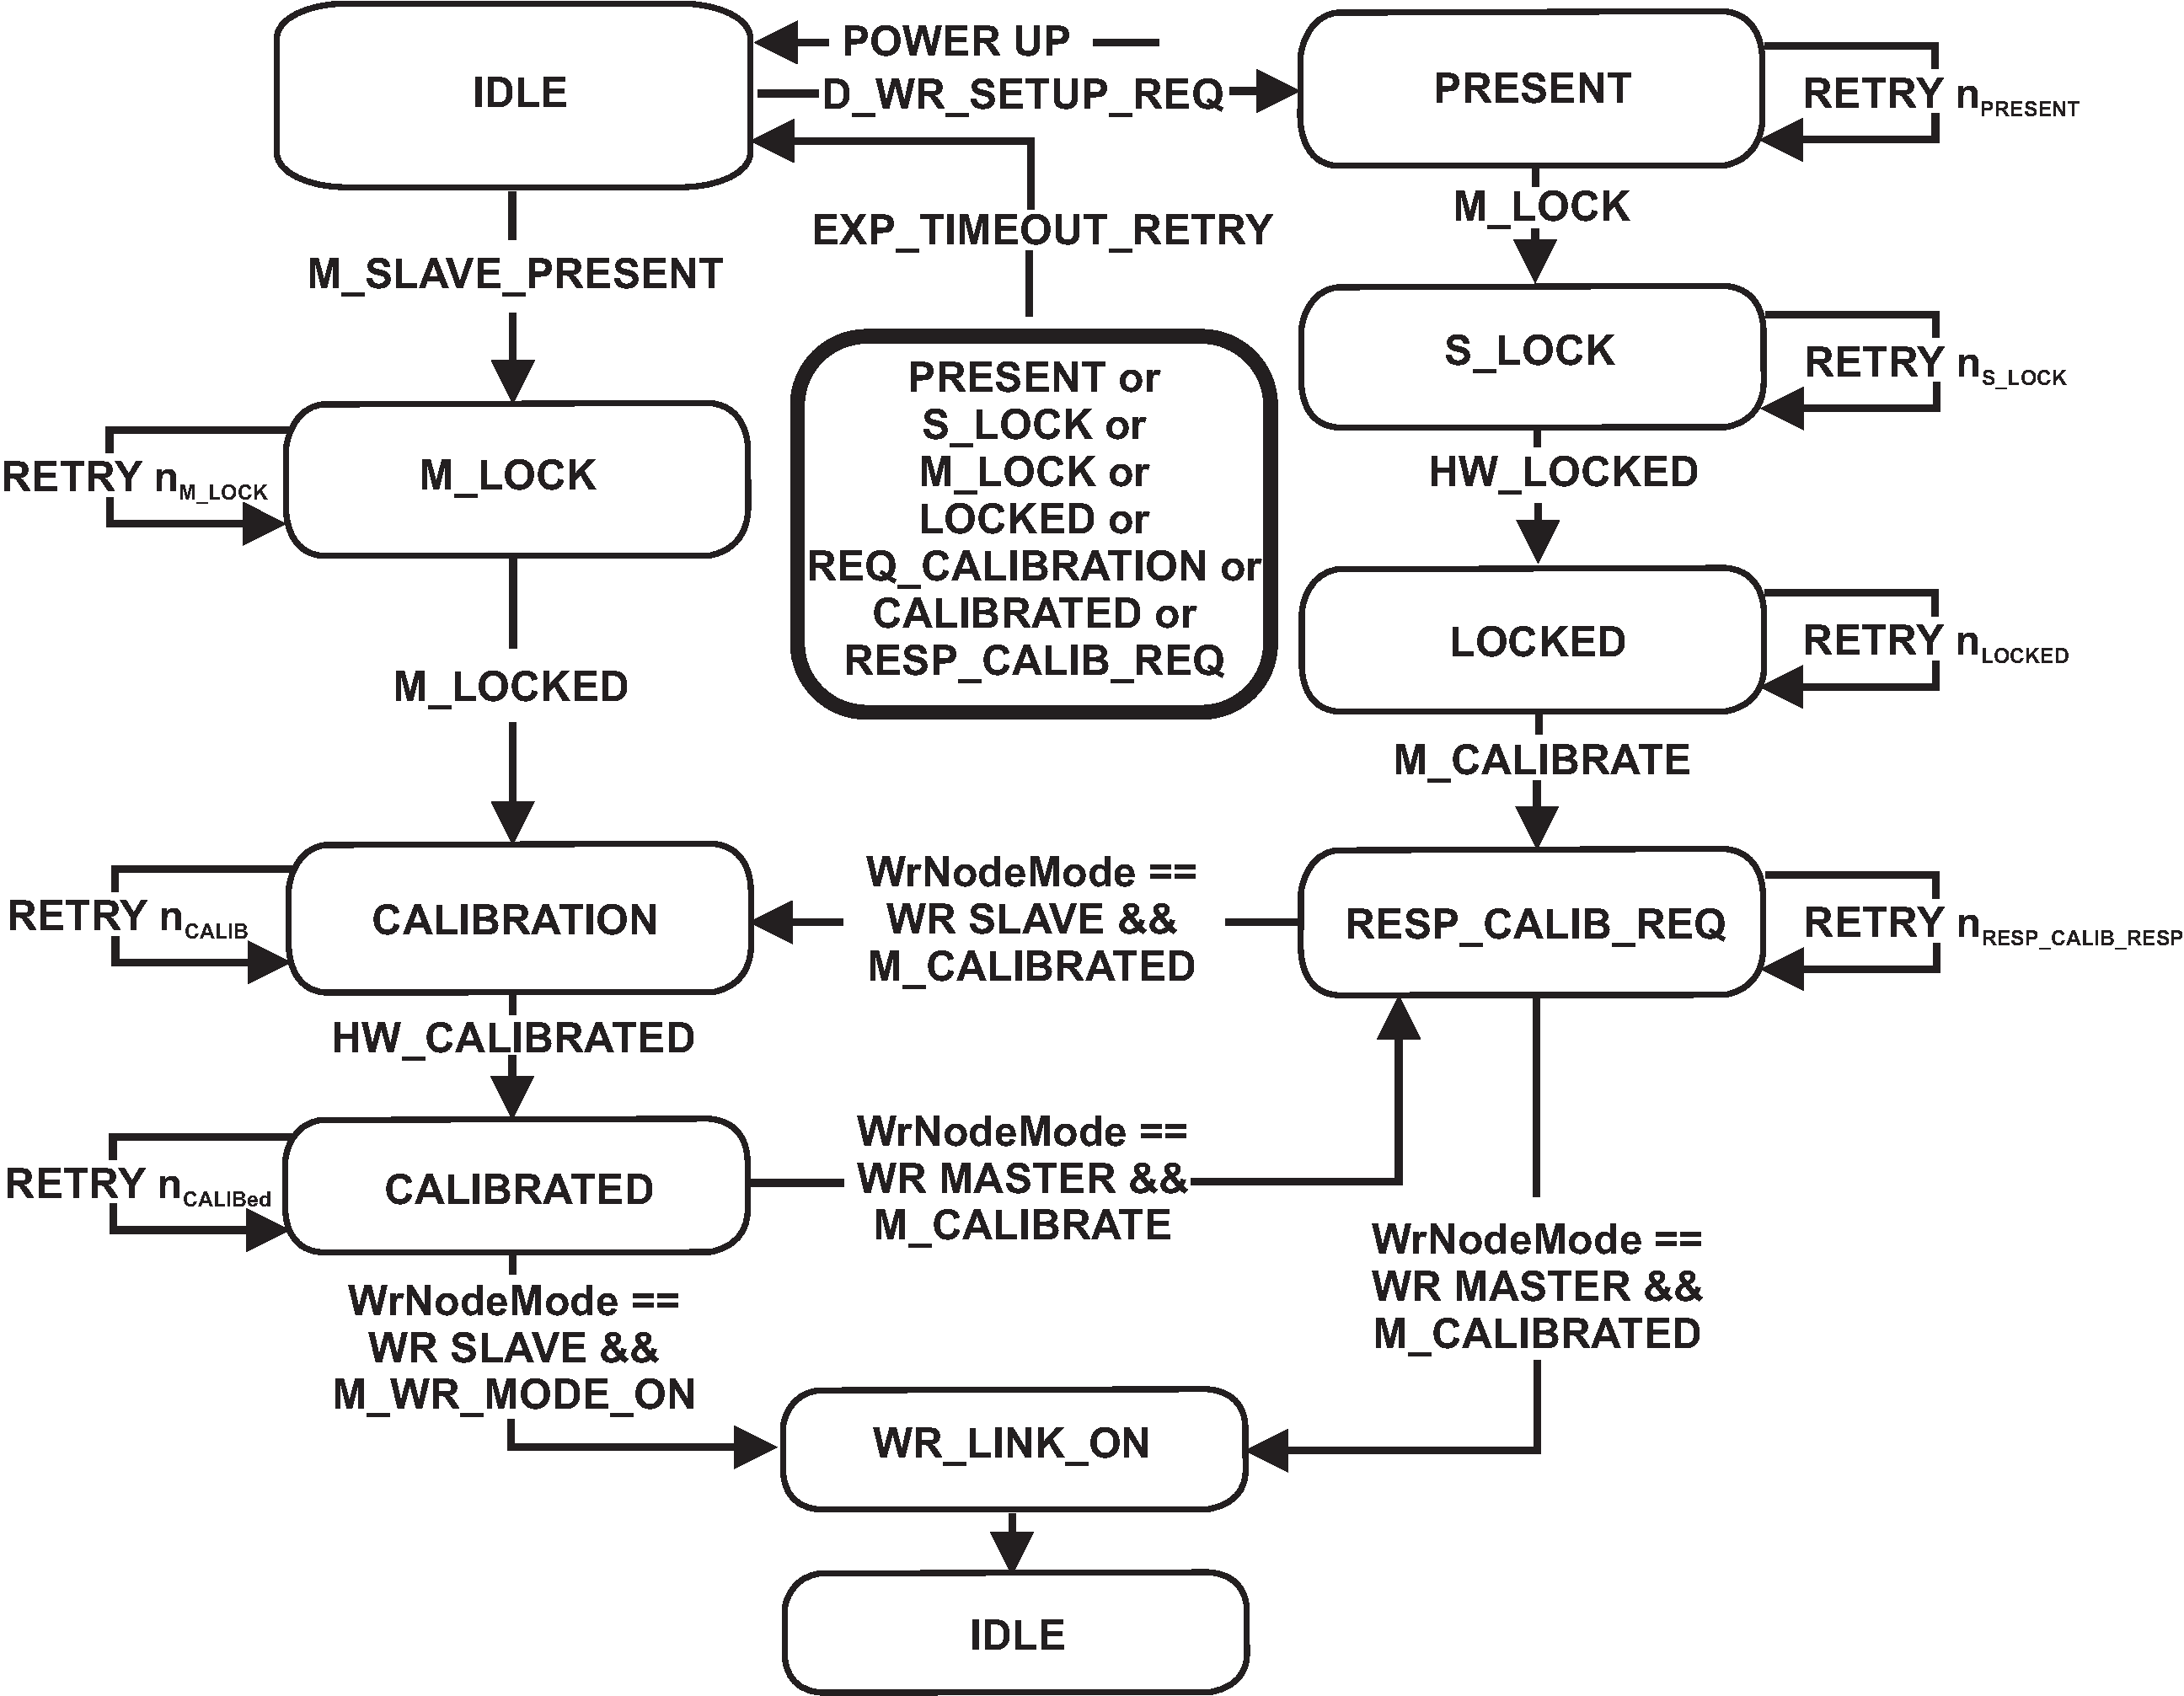
\includegraphics[width=3.1in]{protocol/wrFSM.eps}
\caption{\modified{WR state machine \cite{biblio:WRPTP}.}}
\label{fig:wrFSM}
\end{figure}
%%%%%%%%%%%%%%%%%%%%%%%%%%%%%%%%%%%%%%%%%%%%%%%%%%%%%%%%%%%%%%%%%%%%%%%%%%%%%%%

A WR port can become a WR Master, Slave or enter non-WR mode depending on its 
place in the network hierarchy (mBMC's outcome) and WR-specific parameters. 
The following conditions need to be fulfilled by a WR port 
to enter the WR Slave mode and start the WR Link Setup by entering the PRESENT state of the WR FSM
(\figurename~\ref{fig:wrptpMSGs} \& \figurename~\ref{fig:wrFSM}: \textit{D\_WR\_SETUP\_REQ}):
\begin{itemize}
\item the port is not in the PTP\_SLAVE state \textbf{AND}
\item the port is WR Slave-enabled \textbf{AND}
\item the mBMC's Recommended State is BMC\_SLAVE \textbf{AND}
\item the parent port is WR Master-enabled \textbf{AND}
\item at least one of the ports on the link is not in active WR mode.
\end{itemize}
Similarly, the following conditions need to be fulfilled by a WR port 
to become the WR Master and start the WR Link Setup by entering the S\_LOCK state of the WR FSM
(\figurename~\ref{fig:wrptpMSGs}):
\begin{itemize}
\item the port is in the PTP\_MASTER state \textbf{AND}
\item the port is WR Master-enabled \textbf{AND}
\item the M\_SLAVE\_PRESENT message has been received.
\end{itemize}

On successful completion of the \textit{WR Link Setup} the WR mode (wrMode) 
of a port is validated by setting \\ wrModeOn~=~TRUE. 



%%%%%%%%%%%%%%%%%%%%%%%%%%%%%%%%%%%%%%%%%%%%%%%%%%%%%%%%%%%%%%%%%%%%%%%%%%%%%%%
%             WR PTP Profile
%%%%%%%%%%%%%%%%%%%%%%%%%%%%%%%%%%%%%%%%%%%%%%%%%%%%%%%%%%%%%%%%%%%%%%%%%%%%%%%

\subsection{WRPTP Profile}

\begin{table}[!t]
\caption{WRPTP profile.}
\centering
\begin{tabular}{| c | p{5cm} |}          					\hline
%\multicolumn{2}{|c|}{\textbf{PTP Profile}}  				  \\ \hline
profleName           &  White Rabbit     				  \\ \hline
profileVersion       &  1.0               				  \\ \hline
profileIdentifier    &  08-00-03-00-01-00 				  \\ \hline
organizationName     &  European Organization for Nuclear Research (CERN) \\ \hline
sourceIdentification &  http://www.ohwr.org/projects/white-rabbit         \\ \hline
\end{tabular}
\label{tab:wrPtpProfile}
\end{table}


The White Rabbit PTP profile defines the profile's identification 
(\tablename~\ref{tab:wrPtpProfile}). It specifies the values of some of the parameters
(e.g. priority1, logSyncInterval) and the options to be used. 
It indicates the delay request-response mechanism as the only one used by
the WRPTP. It also specifies the mBMC to be used and the WR TLV to be supported.









%%%%%%%%%%%%%%%%%%%%%%%%%%%%%%%%%%%%%%%%%%%%%%%%%%%%%%%%%%%%%%%%%%%%%%%%%%%%%%%
%             Hardware support
%%%%%%%%%%%%%%%%%%%%%%%%%%%%%%%%%%%%%%%%%%%%%%%%%%%%%%%%%%%%%%%%%%%%%%%%%%%%%%%
\section{WR Hardware Support}
\label{sec:hwSupport}

SyncE is responsible for clock syntonization in the WRN. In the SyncE scheme, the 
reference clock (125MHz) is used to encode the outgoing data
stream. The same clock is retrieved on the other side of the physical
link using the \textit{Clock Recovery System} (CRS, section~\ref{sec:wrCRS}). 
Having the same frequency allows us to use phase detector technologies as a means of evaluating
delays. WR implements Digital Dual Mixer Time Difference (DDMTD) \cite{biblio:WRproject}
phase detection. The measurement of phase is used for 
increasing the precision of timestamps beyond the resolution allowed by the 125MHz clock.
This process \modified{is} described in the next section. 
The DDMTD phase detection is also used to obtain 
\textit{the transmit/receive (Tx/Rx) latencies} (section~\ref{sec:TxRxLatencies})
\modified{and compare frequencies in the CRS}.

%%%%%%%%%%%%%%%%%%%%%%%%%%%%%%%%%%%%%%%%%%%%%%%%%%%%%%%%%%%%%%%%%%%%%%%%%%%%%%%
%             timestamps and fine delay
%%%%%%%%%%%%%%%%%%%%%%%%%%%%%%%%%%%%%%%%%%%%%%%%%%%%%%%%%%%%%%%%%%%%%%%%%%%%%%%


\subsection{Fine Delay Measurement}
\label{sec:fineDelay}
We call \textit{Fine Delay Measurement} the process during which the DDMTD-detected round-trip phase
shift ($phase_{MM}$ in \figurename~\ref{fig:wrLink}) is used to enhance 
timestamp precision and to calculate the precise round-trip delay 
($delay_{MM}$). 
During the fine delay process only the reception timestamp ($t_2$, $t_4$) 
measurements need to be improved as they are transmitted and timestamped in
different clock domains.

A basic timestamp (to be enhanced) is obtained by the detection of 
the Start-of-Frame Delimiter (SFD) in the Physical Coding Sublayer (PCS).
In order to acquire a precision-improved timestamp, we need to eliminate the possible 
$\pm$~1~LSB error \modified{(8ns)} %Pablo's remark to add unit
due to jitter of clock signals and clock-domain crossing. 
Therefore, the Time-Stamping Unit (TSU) produces timestamps on both the rising 
and falling edges of the clock, and later in the process one of them is chosen.
The process involves three steps (see \cite{biblio:TomekMSc} for details):
% \begin{figure}[!t]
% \centering
% \includegraphics[width=2.5in]{fig/preciseTimestamp.ps}
% \caption{Timestamp enhancing \cite{biblio:TomekMSc}.}
% \label{fig:preciseTimestamp}
% \end{figure}
% % Only the reception timestamps ($t_2$, $t_4$)
% need to be enhanced as they are transmitted and timestamped in
% different clock domains. 
%(see \figurename~\ref{fig:preciseTimestamp} for $t_{4}$ to $t_{p4}$
%enhancement explanation)
\begin{enumerate}
   \item rising/falling edge timestamp choice ($t_f$ or $t_r$),
   \item calculating the picosecond part, checking
         its sign and adding a clock period if necessary,
   \item extending timestamps with the picosecond part ($t_{2p}$, $t_{4p}$).
 \end{enumerate}
The modified timestamps are used to calculate the precise round-trip delay
(\figurename~\ref{fig:wrLink}):
\begin{equation}
  \label{eq:delaymm}
  delay_{MM} = (t_{4p}-t_{1}) - (t_{3}-t_{2p})
\end{equation}



%%%%%%%%%%%%%%%%%%%%%%%%%%%%%%%%%%%%%%%%%%%%%%%%%%%%%%%%%%%%%%%%%%%%%%%%%%%%%%%
%             WR Clock Recovery System
%%%%%%%%%%%%%%%%%%%%%%%%%%%%%%%%%%%%%%%%%%%%%%%%%%%%%%%%%%%%%%%%%%%%%%%%%%%%%%%

\subsection{\modified{Robust} Clock Recovery System}
\label{sec:wrCRS}

\begin{figure}[!t]
\centering
%\includegraphics[width=2.95in]{fig/wrCRS.eps}
\includegraphics[height=0.95in]{robustness/wrCRS.eps}
\caption{\modified{White Rabbit Clock Recovery System.}}
\label{fig:PLL}
\end{figure}

The White Rabbit implementation of the CRS (WR CRS) is explained in
detail in \cite{biblio:TomekMSc}, \figurename~\ref{fig:PLL} presents
a very simplified overview of the WR CRS. It is designed to accommodate
multiple sources of frequency (physical links) with a single source
being used (active) at a given time. A seamless switching of the
active source is one of the goals of the design to enable network
topology redundancy \modified{and, as a consequence, offer robust and stable synchronization 
(see section~\ref{sec:wrBMC})}.


All input reference clocks (\textit{ref clk}) and a feedback clock (\textit{feedback clk}) are
fed into DDMTD and degliching units (\textit{DDMTD}). The input clocks are mixed by the DDMTDs with 
the offset frequency (\ref{equation:offsetFreq}) which is derived from the 
active ref~clock. The frequency-mixing results in a low frequency clock signal which maintains the
original 
phase shift. 
\begin{equation}
  \label{equation:offsetFreq}
     f_{offset}[ns] =  125[MHz] * \frac{2^N}{2^N+ \Delta}% \mbox{ , }N=14 \mbox{ \& } \Delta=1
\end{equation}
A prototype implementation using $N=14$ and $\Delta=1$ has demonstrated satisfactory performance 
\cite{biblio:TomekMSc}. Each output of the DDMTD reference channel is compared with the output
of the feedback channel in the \textit{phase and frequency error detection} units. The additional 
input to the units is the \textit{WRPTP phase shift} obtained in the \textit{Fine Delay
Measurement}. The phase and frequency error (\textit{phase and freq error}) between the feedback
clock and each reference clock, corrected by WRPTP phase shift, is calculated and fed into the
multiplexer (\textit{MUX}).
During normal operation, the active reference clock (from the Primary Slave port, 
section~\ref{sec:wrBMC}) is used to feed the PI controller and produce the output reference signal.
However, if the malfunction of the active ref clock is detected, the switch-over process
takes place: the MUX is switched to feed the PI with the error data from another reference channel
(from the Secondary Slave port).
\modified{An estimate of the average phase and frequency errors can be provided to the PI controller
to improve hold-over performance if all the reference channels fail.}



The active clock malfunction takes 3 consecutive invalid symbols
($\sim24ns$) to detect while the phase and frequency error detection is performed
at a low frequency (kHz). Therefore, the continuity of the synchronization is 
guaranteed during the switch-over. 



%%%%%%%%%%%%%%%%%%%%%%%%%%%%%%%%%%%%%%%%%%%%%%%%%%%%%%%%%%%%%%%%%%%%%%%%%%%%%%%
%             Tx/Rx calibration
%%%%%%%%%%%%%%%%%%%%%%%%%%%%%%%%%%%%%%%%%%%%%%%%%%%%%%%%%%%%%%%%%%%%%%%%%%%%%%%

\subsection{The transmit/receive (Tx/Rx) latencies} 
\label{sec:TxRxLatencies}

\begin{figure}[!t]
\centering
%\includegraphics[width=1.74in]{fig/calibration.eps}
\includegraphics[height=0.95in]{misc/calibration.eps}
\caption{\modified{Rx/Tx latency measurement \cite{biblio:WRPTP}. }}
\label{fig:calibration}
\end{figure}

The transmit/receive (Tx/Rx) latencies in most PHYs vary for
each \modified{Phase-Locked Loop/Clock Data Recovery (PLL/CDR)} 
%\modified{PLL/CDR\footnote{\modified{Phase-Locked Loop/Clock Data Recovery}}} 
lock cycle, but stay constant once the PHY is
locked. This is the case of the PHY used in the WR Switch prototype
(TCK1221), therefore an Tx/Rx latency measurement is required. Tx
latency is measured by feeding the transmit path with a sequence of
RD+ K28.7 code-group (Appendix~36A.2 of \cite{biblio:IEEE8023}). 
Such signal creates a 125MHz clock on
the SerDes I/O. Since the Tx clock frequency is also 125MHz, the DDMTD
can be used to measure the phase shift between the SerDes I/O and the
Tx clock, effectively measuring Tx latency. By receiving the K28.7
signal from the link partner, the Rx latency can be measured using the
same method. This process, depicted in \figurename~\ref{fig:calibration},
is performed during the WR Link Setup (section~\ref{sec:wrLinkSetup}).




%\section{Clock Resilience}

While the previous chapter described WRPTP focusing on a single
Master-to-Slave link, clock resilience needs to be considered in terms
of the entire WR Network.

\subsection{Clock Path redundancy}

In a WRN, the clock is distributed along so-called \textit{clock
  paths}. A path is understood as the cables and switches by which
information is sent from the transmitter (node/switch) to the receiver
(switch/node). The continuity of clock distribution -- existence of
clock paths to all WRN components -- is essential in ensuring clock
resilience. Therefore, clock path redundancy is introduced. This
allows to prevent a \textit{single point of failure} \footnote{Failure
  of a single network component.} from affecting clock distribution
and inevitably translates into network topology redundancy, which is
supported by the \textcolor{red}{WR Switch}. The \textcolor{red}{WR
  Switch V2 (WRSv2)} has two uplinks which can be connected to
separate sources of timing (downlinks of other \textcolor{red}{WR
  Switches} or a node being \textit{grandmaster}). Redundancy of the
WRN is limited by a number of factors:
\begin{itemize}
\item Latency of data delivery which limits the number of network
  layers.
\item SyncE which enforces a tree-like network structure and ensures
  high-quality frequency distribution only through a limited number of
  switches.
\item Data delivery reliability which enforces a tree-like topology
  with the roles of ports defined \textit{a priori} by the Rapid
  Spaning Tree Protocol (RSTP) algorithm (\cite{biblio:IEEE8021D},
  \cite{biblio:Robustness}).
\end{itemize}
Studies (\cite{biblio:Robustness}) suggest that, given the limitations
in topology, the two uplinks of WRSv2 might be not sufficient to
achieve high network reliability. The next version of the
\textcolor{red}{WR Switch (WRSv3)} will eliminate this limitation.

The choice of an active clock path -- the uplink which is used for
syntonization and synchronization -- is made based on the RSTP
algorithm.

\subsection{Switch-over}

The redundancy of clock path ensures continuity of clock distribution
but introduces a possible instability of the recovered clock during
the process of switching between sources (active uplink), further
called \textit{switch-over}. Syntonization and synchronization are
governed by SyncE and WRPTP respectively.  Therefore, both need to
take account of stability during \textit{switch-over}.

\subsubsection{SyncE-wise}

The White Rabbit clock recovery unit (described in
Sec.~\ref{sec:hwSupport}), by design, enables multiple inputs (RX
clocks). The phase and frequency errors of all the input clocks are
continuously tracked and fed into the VCTCXO control algorithm and a
\textcolor{red}{delay can be introduced to wait for freqency/phase
  error validation}, if tests show such a need. Therefore, SyncE-wise
switch-over is considered seamless for syntonization.
\textcolor{blue}{I would need some numbers and tests here}

\subsubsection{WRPTP-wise}

Since a WRN is a set of independent M-to-S link connections, WRPTP is
unaware of whether a given link is active or not. Delay and offset
measurements are performed on all the links all the time and the
information is provided to the clock recovery unit (see
\figurename~\ref{fig:PLL}). Therefore, the switch-over is unnoticible
for WRPTP and shall be seamless for synchronization.
\textcolor{blue}{ Measurement of "backup" offset and delay with
  reference to the primary one - idea by Tomek to further decrease
  switch-over instability }

\subsection{External conditions variation}

Apart from the switch-over process, another potential source of clock
instability is a variation of external conditions,
e.g. temperature. It affects the characteristics of the physical
connections, consequently changing the delay introduced by the medium
--the variable delay ($\delta_{ms,sm}$).  It is important to note that
frequency distributed over SyncE is not affected by this
phenomenon. Therefore, only synchronization over WRPTP, i.e. delay
change, needs to be compensated. This is done by periodically
measuring the delay through a standard exchange of PTP messages. The
frequency of measurements needs to be greater then the speed of
temperature changes, which is reasonably slow.
\textcolor{red}{Therefore, a much lower rate of message exchange than
  in standard PTP is sufficient.}

\subsection{Loss of WRPTP-messages}

PTP employs timeouts to address PTP-specific message loss, provoking
repetition of operations and re-sending of messages. WRPTP uses the
same idea during the \textit{WR Link Setup} (see
Sec.~\ref{sec:wrLinkSetup}) repeating operations and re-sending WR
management messages in case of message loss. The measurement of the
offset and delay in WRPTP is much more tolerant to multiple message
loss. Unlike standard PTP, WRPTP is responsible only for
synchronization (syntonization is done through SyncE). After achieving
synchronization with the master at the beginning of the connection,
the offset changes only due to temperature-related delay
variation. The rate of delay measurements through the PTP-message
exchange is supposed to be much greater than the rate of change of
physical medium parameters. Therefore, multiple PTP-message loss is
tolerated with no effects on clock stability.  \textcolor{blue}{we
  should probably have a sanity check in the PTP daemon for ruling out
  impossible corrections, i.e. very fast changes probably due to a
  measurement or transmission error}

\subsection{Cascading Boundary Clocks}

A switch can be seen as a boundary clock. In standard PTP, a cascade
of boundary clocks faces nonlinear decreasing synchronization accuracy
problems due to error accumulation.  \textcolor{blue}{
  \begin{itemize}
  \item if it is possible to make measurements (we need $\geq$ 3
    switches), measurements here
  \item the deterioration should be due to SyncE...
  \item measurements would answer the question: how many layers of
    switches we can have.
\end{itemize}
}

\section{Test Results}

In order to test the performance of time and frequency transfer, the 
test setup depicted in \figurename~\ref{fig:testSetup} was assembled.
The system consists of 4 switches connected with 5km bare fiber rolls in 
a daisy chain (15~km total). Varying operating conditions were simulated
by heating the fiber with a hot air gun. 


\begin{figure}[!t]
\centering
%\includegraphics[width=2.0in]{fig/measSystem.ps}
\includegraphics[width=1.6in]{measurements/measSystem.ps}
\caption{Test setup.}
\label{fig:testSetup}
\end{figure}

%\subsection{Syntonization}

The frequency transfer performance was evaluated using an Agilent E5052B signal source analyzer. 
A cesium clock served as a source of 10~MHz reference frequency for the master.
The Power Spectral Density (PSD) of the phase noise of the master and each slave 
REF clocks was determined. The integrated jitter from 10Hz to 40~MHz measured on each 
slave is presented in Table~\ref{tab:freqTransfer}. The jitter on a single link is below 2~ps. 
%the accumulation effect of cascaded switches can be observed.

The accuracy \modified{and precision} of synchronization %was 
were characterized by measuring the skew between 
the master and each slave clock signal over a period of 1 hour with a LeCroy oscilloscope
(Table~\ref{tab:freqTransfer}). A histogram of master-slave offsets constructed from the obtained
samples is depicted in \figurename~\ref{fig:offset}. The single link skew is
well below 1~ns. In this particular case, the skews of the first and second link cancel,
therefore the skew between the master and the last slave is below 200~ps. However, if the
cancellation did not take place, the accumulated skew would be still below 0.5~ns. The varying
conditions introduce only a transient increase of the skew's standard deviation (sdev) of 
$\sim$~5~ps. This is a consequence of the purposely %very 
low exchange-rate of PTP messages (1~s), compared
to the fast heating provided by the hot air gun.
\begin{figure}[!t]
\centering
%\includegraphics[width=2.3in]{fig/cascadedMeas.eps}
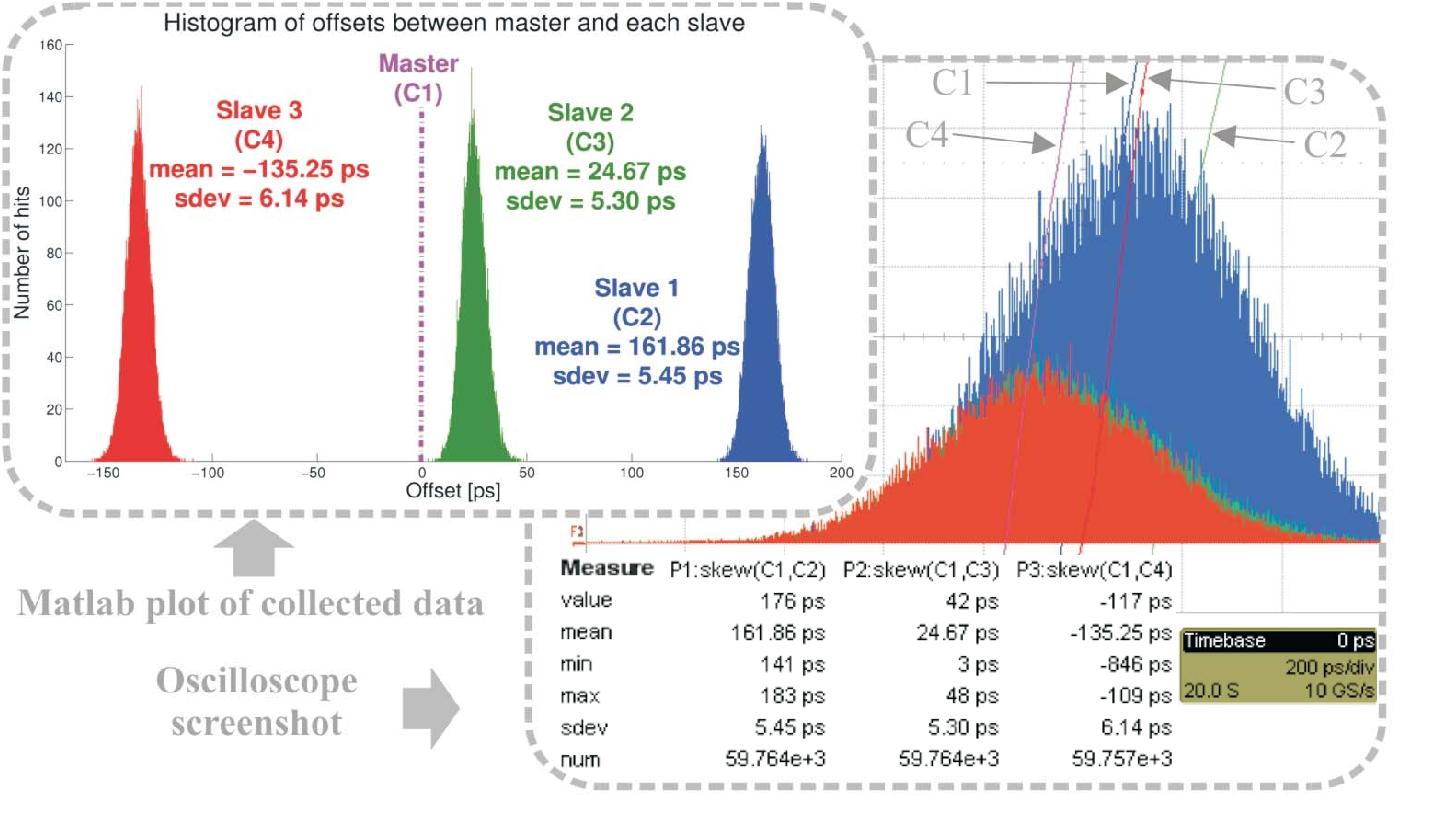
\includegraphics[width=3.4in]{measurements/measResults-new.eps}
\caption{\modified{Synchronization performance.}}
\label{fig:offset}
\end{figure}

\begin{table}[!t]
\caption{Synchronization and syntonization performance.}
\centering
\begin{tabular}{| c | c |c | c |}          \hline
\multirow{2}{*}{\textbf{Switch}}& 
\textbf{Integrated jitter [ps]}& 
\multicolumn{2}{|c|}{\textbf{Offset [ps]}}  \\ \cline{2-4}
%&   \\ \hline
            & 10Hz-40MHz& mean &  sdev    \\ \hline
            %&   [ps]    &   [ps]     & [ps] & [ps]  & [ps] & [ps]  \\ \hline
1           & 1.6637    &  161.86       &  5.45            \\ \hline
2           & 2.4887    &  24.67        &  5.30            \\ \hline
3           & 2.3025    & -135.25       &  6.14            \\ \hline

\end{tabular}
\label{tab:freqTransfer}
\end{table}


\section{Conclusions}
\label{sec:conclusions}

In this paper the first deployment of a ``beta version" of a White Rabbit
system is described. The deployed system includes a WR Network (consisting of switches) 
interconnecting WR Nodes. 

The results indicate that a system based on the 
White Rabbit technology is capable of providing nanosecond accuracy of synchronization 
over large distances (i.e. over 16 km). The measured accuracy of the deployed system  
is 0.517~ns and the precision is 0.119~ns. The calculated MTIE is below 1.05~ns
with only 0.0003$\%$ of values exceeding the $\pm$0.5~ns range.
The WR-timebase 
guarantees sub-nanosecond accuracy and tens of picoseconds precision of the distributed time 
and frequency reference regardless of the changing temperature conditions. 
The standard deviation of the skew measured between the time reference (grandmaster) and 
the nodes (over a peak-to-peak 45 
degrees Celsius temperature range) is 55~ps while the MTIE is below 342~ps. 
The temperature tests indicate that the acceptable influence   
of the temperature variation of WR devices on the quality of synchronization can be easily
reduced by compensating temperature-induced changes of the hardware delays. 
Such a compensation should be considered in future developments of the WR technology.

The high accuracy and precision time transfer over an Ethernet-based WR Network has many potential
applications. Precise time-tagging of the input events using WR-provided timebase is the first to
be realized. Therefore, the described deployment marks an important milestone in the White Rabbit Project -- 
proof-of-concept technology becomes a working solution. This solution is about to be 
commercially available while sustaining its openness (open hardware and open software). 


\newpage

%
\begin{thebibliography}{9}

\bibitem{IEEE1588}
  IEEE Std 1588-2008
  \emph{IEEE Standard for a Precision Clock Synchronization Protocol for
Networked Measurement and Control Systems}.
  IEEE Instrumentation and Measurement Society, New York,
  2008,
  http://ieee1588.nist.gov/.

\bibitem{IEEE8021D}
  IEEE Std 802.1D-2004
  \emph{IEEE Standard for Local and metropolitan area networks, Virtual Bridged
Local Area Networks}.
  LAN/MAN Standards Committee, New York,
  2006.

\bibitem{IEEE8021Q}
  IEEE Std 802.1Q-2005
  \emph{IEEE Standard for Local and metropolitan area networks Media Access
  Control (MAC) Bridges}.
  IEEE Computer Society, New York,
  2004.

\bibitem{IEEE8023}
  IEEE Std 802.3-2008
  \emph{IEEE Standard for Information technology - Telecommunications and
information exchange between systems - Local and metropolitan area networks -
Specific requirements}.
  IEEE Computer Society, New York,
  2008.

\bibitem{UplinkFast}
  CISCO Document ID: 10575
  \emph{Understanding and Configuring the Cisco UplinkFast Feature}.
  http://www.cisco.com.

\bibitem{SynchE}
  ITU-T G.8262/Y.1362
  \emph{Timing characteristics of a synchronous
  Ethernet equipment slave clock}.
  TELECOMMUNICATION STANDARDIZATION SECTOR OF ITU, 
  07/2010.

\bibitem{WRPTP}
 Emilio G. Cota, Maciej Lipinski, Tomasz Wostowski, Erik van der Bij, Javier
 Serrano
  \emph{White Rabbit Specification: Draft for Comments}.
  CERN, Geneva
  09/2010.

\bibitem{FAIR}
  R.Bar
   \emph{The FAIR Accelerator Control System}
   The excerpt from the updated FAIR Technical Design Report,
   Hamburg,
   2008.
   
\bibitem{DesigningLSLANs}
  Kevin Dooley
  \emph{Designing Large-Scale LANs}
  O'REILLY,
  2002.

\bibitem{HWpresentation}
  Tomasz Wlostowski
  \emph{White Rabbit HW status}
  White Rabbit Developers Meeting, Geneva, CERN
  December 2010,
  http://www.ohwr.org/attachments/404/hw\_pres.odp

\bibitem{PropagationDelay}
  P.P.M. Jansweijer,
  H.Z. Peek
  \emph{Measuring propagation delay over a 1.25 Gbps
         bidirectional data link}
  National Institute for Subatomic Physics, Amsterdam
  May 31, 2010.

\bibitem{FAIRtiming}
   T. Fleck 
   R. Bar 
  \emph{FAIR Accelerator Control System 
        Baseline Technical Report }
  DRAFT,
  Hamburg,
  2009.

\bibitem{CERNtiming}
  Mr. XXX
  \emph{I need some nice doc here :) }
  Current source: Javier + Julian,
  CERN, Geneva,
  xxx.

\bibitem{ciscoRSTP}
  Mr. XXX
  \emph{I read the doc, I cannot find it at the moment }
  CISCO,
  somewhere,
  xxxx.

\bibitem{FAIRtimingSystem}
  T. Fleck, C.Prados, S.Rauch, M.Kreider
  \emph{FAIR Timing System}
  GSI,
  v1.2,
  12.05.2009.

\bibitem{The All-New Switch Book: The Complete Guide to LAN Switching Technology}
 Rich Seifert, James Edwards
 \emph{The All-New Switch Book: The Complete Guide to LAN Switching Technology}
 Wiley Pusblishing, Inc. 

\bibitem{IEEE8021Qbb} 
 \emph{IEEE 802.1Qbb/D2.3. Draft Standard for Local and Metropolitan Area
      Networks - Virtual Bridged Local Area Networks - Amendment XX:
Priority-based Flow Control.}  
   June 9,
  2009.

\bibitem{atm_traffic} 
 \emph{Network Testing Solutions, ATM Traffic Management White paper}

\bibitem{FlowControllers} 
 \emph{... missing citation...}

\bibitem{reed_solomon} 
 \emph{RFC 5510 Reed-Solomon Forward Error Correction (FEC) Schemes}
J. Peltotalo
S. Peltotalo
Tampere University of Technology
April 2009

\bibitem{reed_solomon_theory}
\emph{An Introduction to Galois Fields and Reed-Solomon Coding}
James Westall
James Martin
School of Computing
Clemson University
October 4, 2010

\bibitem{hamming_Codes}
\emph{Hamming Codes}
Charles B. Cameron
Electrical Engineering Department, 
United States Naval Academy
Department of Electrical Engineering .
April 19, 2005

\bibitem{TomekMSc} 
 \emph{Precise time and frequency transfer in a White Rabbit netwokr, MSc
Thesis}
  Tomasz Wlostowski
  Warsaw University of Technology
  To be published.

\bibitem{WRdemo} 
 \emph{White Rabbit DEMO(2)}
  Tomasz Wlostowski,
  Maciej Lipinski
  CERN, Geneva,
  11/2010.

\bibitem{FaultTree} 
 \emph{Reliability Workbench, FaultTree}
  www.Isograph.com.

\end{thebibliography}


\bibliographystyle{IEEEtran}
\bibliography{IEEEabrv,./biblio}

\end{document}


